\section{Introduction}
%
\label{sec:introduction}

The term tides refers to changes in the shape of an astronomical object (in our
case a planet or a star) in response to differences in the gravitational pull of
a nearby mass at different locations within the object. Below, tides and their
effects are discussed qualitatively. For a full mathematical description of
tides see \cite{Murray_Dermott_book}.

Consider an exoplanet system consisting of a single planet orbiting a single
star in a circular orbit. The gravitational acceleration due to the star at the
location of the planet's center provides the centripetal acceleration needed to
keep the planet in orbit. The part of the planet facing the star is closer to
the star and therefore experiences a slightly stronger gravitational pull.
However, if we ignore the rotation of the planet for a moment, that part of the
planet must follow a path with the same radius and period as the center of the
planet (though with its center offset slightly). The result is that the star
provides larger gravitational acceleration to that part of the planet than the
required centrifugal acceleration. This excess force as referred to as the tidal
force, and it is directed towards the star for the star-facing part of the
planet. Similarly, on the far side of the planet, the star's gravity is slightly
smaller than what is required to keep that part of the planet in orbit,
resulting in a tidal force pointing away from the star. These tidal forces cause
the planet to elongate along the star-planet line, and squeeze in the
perpendicular direction. This elongation is frequently referred to as the tidal
bulge.

Let us now consider the rotation of the planet. If the period of rotation is
exactly equal to the orbital period (a.k.a. synchronous rotation), the
sub-stellar point is fixed on the planet's surface, and consequently the tidal
bulge is also fixed relative to the planet. However, if the rotation and orbital
periods differ, the tidal bulge will travel on the planet's surface. If the
rotational angular velocity of the planet is $\Omega_{pl}$, and the orbital
angular velocity is $\Omega_{orb}$, a point on the surface of the planet will
travel at a rate of $\Omega_{orb} - \Omega_{pl}$ relative to the sub-stellar
point. Since there are two tidal bulges on the planet (one on the side facing
the star and one on the opposite side), the planetary material will experience a
tidal wave with a frequency of $2(\Omega_{orb} - \Omega_{pl})$.

Any time dependent deformation of the planet will result in some conversion of
mechanical energy to heat. The simplest picture of this is friction between
parts of the planet that move relative to each other. For a continuous medium,
this friction is encapsulated in the concept of viscosity. However, a great
variety of physical processes can result in energy dissipation of tidal
perturbations. The physical causes and the amount of energy that is dissipated
depends on the internal structure and properties of the planet.

Regardless of the causes, this energy dissipation introduces a delay between the
tidal forcing and the response of the planet to that forcing. If the planet
spins faster than synchronous (i.e.  $\Omega_{pl} > \Omega_{orb}$), the tidal
bulge will be ahead of the sub-stellar point, and if $\Omega_{pl} <
\Omega_{orb}$, the tidal bulge will lag behind (Fig.~\ref{fig:tidal_bulge}).

\begin{figure}[t]
%
    \centering
%
    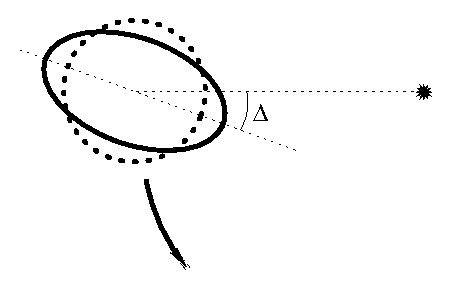
\includegraphics[width=0.5\textwidth]{tidal_bulge.eps}
%
    \caption{
%
        Exaggerated tidal bulge on a planet orbiting a star. Assuming that the
        planet spin angular velocity is smaller than than the orbital angular
        velocity, the tidal bulge will lag behind the sub-stellar point by an
        angle $\Delta$.
%
    }
%
    \label{fig:tidal_bulge}
%
\end{figure}

The two tidal bulges, now shifted relative to the star-planet line, will
experience the gravitational pull of the star. Since the closer bulge will feel
a stronger gravitational force than the farther bulge, there will be a net
torque on the planet. If the bulge is carried ahead of the sub-stellar point by
rotation, the gravitational pull of the star will apply a torque to the planet
opposite to its rotation, acting to slow down its spin, and the reaction force
on the star will act to add angular momentum to the orbit. Conversely, if the
tidal bulge lags behind the sub-stellar point, the gravitational pull of the
star will act to spin the planet up, taking angular momentum out of the orbit.

The discussion above assumed that the equator of the planet is aligned with the
orbital plane. This is not necessarily the case. If the planet's spin is tilted
with respect to the orbit, regardless of whether the planet is rotating faster
or slower than the orbit, rotation will shift the bulges away from the
sub-stellar point. This in turn will result in a torque that will tend over time
to bring the planet's equator and the orbital plane into alignment.

So far we only considered circular orbits. For non-circular orbits, the orbital
angular velocity is no longer constant. It is highest near periapsis (closest
approach between the planet and star) and lowest near apoapsis (largest
planet-star distance). In this case, tides will push the spin of the planet to a
state where the average torque over an orbit vanishes. This is known as
pseudo-synchronous rotation. Near periapsis the orbital angular velocity is
smaller than the pseudo-synchronous spin of the planet, thus the tidal bulge
leads the sub-stellar point, causing angular momentum to flow from the planet to
the orbit. Then for the part of the orbit around periapsis, the orbital angular
velocity exceed the pseudo-synchronous spin of the planet, causing angular
momentum to flow in the opposite direction. Since tides are stronger near
periapsis, the pseudo-synchronous period is somewhat shorter than the orbital
period, resulting in the planet being spun-down over a larger fraction of the
orbit, but at a slower rate.

For eccentric orbits, even if the planet is pseudo-synchronized, tidal
dissipation does not vanish, because the planet-star distance varies over time,
and the sub-stellar point is not fixed on the surface. From the discussion about
pseudo-synchronous period above, it is evident that near periapsis, the
sub-stellar point will drift eastward, and near apoapsis it will drift westward,
with a long-term westward average, since the pseudo-synchronous spin period is
shorter than the orbital period. These shifting both in location and amplitude
tidal bulges will still experience friction. Thus while no angular momentum will
be exchanged between the planet and the orbit, energy will be extracted from
the system and dissipated as heat, causing the orbit to circularize over time.

Everything we have said so far about the tides the star raises on the planet
applies equally to the tides the planet raises on the star. For circular orbits,
aligned with the stellar equator, if the spin angular velocity of the star
exceeds the orbital angular velocity, angular momentum is transferred from the
stellar spin to the orbit, and if the stellar spin is slower than the orbit,
angular momentum flows in the opposite direction. Similarly, we can define a
pseudo-synchronous period for the star at which the net tidal torque averaged
over a complete orbit vanishes. Even if the star is spinning
pseudo-synchronously, tidal energy dissipation continues and acts to circularize
the orbit over time. For misaligned orbits, tides will gradually work to align
the orbital plane with the stellar equator.

The amplitude of the tidal bulge is set by competition between the tidal force
and the self-gravity of the planet or the star experiencing the tides.
Consequently, the planetary tides are positively correlated with the planet
radius and stellar mass and negatively correlated with the planet mass.
Conversely, the stellar tides are larger the larger the mass of the planet.
Finally, both stellar and planetary tides get weaker with increasing
star-planet separation, implying that tides will only be important if the planet
gets close to its parent star for at least some part of its orbit. This can
occur in one of two ways: either the planet has a very small orbital semimajor
axis (short period orbit), or the eccentricity of the planet is very large
making the pericenter distance small.

\section{Tidal timescales}

Based on the discussion above, we can think of four separate tidal evolution
timescales:

\begin{enumerate}
%
    \item The timescale on which the planet's spin gets pseudo-synchronized and
        aligned with the orbit
%
    \item The timescale on which the orbit circularizes
%
    \item The timescale on which the orbital period of a circular orbit changes
%
    \item The timescale on which the stellar spin changes
%
\end{enumerate}

In order to compare some of these timescales, we need to consider the relative
angular momenta of the planet's spin, the orbit, and the stellar spin.

The planet's spin angular momentum is negligible compared to both the orbital
angular momentum and the spin angular momentum of the star.  Consequently, both
the direction and period of the planet's spin can be changed by tides without
significantly affecting the orbit, implying that the timescale on which the
planet's spin gets pseudo-synchronized and aligned with the orbit is negligible
compared to the timescales on which the orbit or the stellar spin evolve. Thus,
we can assume that if a given exoplanet orbits close enough to its star for
tides to be important, to a good approximation we can assume that the planet's
spin is aligned with the orbit and pseudo-synchronized.

To compare the two timescales on which the orbit changes, we begin by comparing
the importance of the planetary to the stellar tides. The tidal deformation of
an object is set by a competition between the tidal force due to the companion
and the self-gravity of the object being tidally stretched. Since the planet has
a smaller self-gravity and experiences much larger tidal force than the star,
the planet is much more tidally deformed than the star. Consequently, as long as
planetary tides are not static they will drive faster orbital evolution than the
stellar tides. By the reasoning above, for both circular and eccentric orbits,
we expect the planet to be aligned and spin pseudo-synchronously with the orbit.
Hence, for eccentric orbits, the planetary tides still contribute to the
evolution, while for circular orbits they do not. This in turn means that the
tidal circularization timescale is shorter than the timescale on which circular
orbits change their period, since the latter is only driven by the much weaker
stellar tides.

To compare these timescales to the timescale on which the stellar spin is
affected by tides, note that stars have sufficiently large moment of inertia
for their spin angular momentum to be comparable to or larger than the orbital
angular momentum. Since only the stellar tides can affect the stellar spin, this
implies that the timescale on which the stellar spin changes is comparable to or
longer than the timescale on which the orbital period changes.

\section{Equilibrium state}
%
\label{sec:equilibrium}

Let us significantly simplify the problem of tidal evolution. First, let us
stick to a system with just a planet and a star. Second, let us assume that
tides are allowed unlimited time to act. Third, let us ignore all other
processes that can change the system. Under these conditions, one of two
possible final states will eventually be reached. Either the two objects will
merge, or the system will end up in a circular orbit, the planet and stellar
spin axes will be aligned with the orbital angular momentum, and the planet and
star spin periods will be equal to the orbital period.

Which of these two possibilities the system approaches depends on the initial
angular momentum available to the system. Since tides are purely internal
interactions within the system, they can only redistribute angular momentum, but
the total angular momentum vector must remain fixed. Let $M_\star$ and $M_p$ be
the masses of the star and planet, and $I_\star$ and $I_p$ their moments of
inertia.

If the two objects are to avoid merging, and reach a final synchronized spin in
a circular orbit with semimajor axis $a_f$, the final spin angular velocities of
both the star and the planet must be equal to the orbital angular velocity,
which by Kepler's third law is:

\begin{equation}
%
    \Omega_{orb} = \sqrt{\frac{G (M_\star + M_p)}{a_f^3}}
%
\end{equation}

This gives the final angular momentum of the system as:

\begin{equation}
%
    L
%
    =
%
    \left(I_\star + I_p) \sqrt{\frac{G (M_\star + M_p)}{a_f^3}}
%
    +
%
    M_\star M_p \sqrt{\frac{G a_f}{M_\star + M_p}}
%
    \label{eq:equilibrium_angmom}
%
\end{equation}

The last term above is the orbital angular momentum.

From the above equation we see that $L \rightarrow \infty$ as $a_f \rightarrow
0$, and $a_f \rightarrow \infty$, and $L$ has a minimum at a finite value of
$a_f$. Figure \ref{fig:equilibrum_angmom} shows a graph of Eq.
\ref{eq:equilibrium_angmom} for a Jupiter mass planet around a Solar mass star.

If the initial angular momentum is smaller than this critical value, no
equilibrium state exists with the two objects surviving, hence the ultimate fate
of a system starting below this critical angular momentum is for the planet to
be engulfed by the star. If the initial angular momentum is larger than the
minimum angular momentum required by the final equilibrium state, then Eq.
\label{eq:equilibrium_angmom} allows us to calculate the final semimajor axis
and in turn the spin periods of the planet and the star.

In practice, the simplifying assumptions we made above are often violated. Many
exoplanet systems have multiple planets, or even multiple stars. These extra
objects can perturb the orbit, maintaining non-zero eccentricity in spite of
tides. A particularly common situation that arises involves a pair, or more
planets in what are called low order mean motion resonances. This mouthful of a
term refers to the situation where a small integer times the orbital period of
one planet is very close to another small integer times the orbital period of
another planet. An example of such mean motion resonance in our own solar system
are three of the four major satellites of Jupiter, where the orbital periods of
Io, Europa, and Ganymede are in a 1:2:4 ratio. Because planets in such
configurations repeatedly get closest to each other in the same place in their
orbit, the gravitational interactions between such planets are particularly
effective in exciting their orbital eccentricities. This excitation can compete
with tidal circularization, maintaining non-zero eccentricity. This prevents
tides from achieving the above equilibrium state. Instead, it can be shown
mathematically that in many situations, as tidal dissipation removes energy from
the systems, the resonant chain of planets will be maintained, causing all
planets to migrate inward together. This could cause the eventual engulfment of
some of the planets by the star even if the initial angular momentum is
sufficient according to the above criterion. In our own solar system, this
common migration seems to occur for Io, Europa, and Ganymede. Except in this
case the system of satellites moves outward rather than inward, because
Jupiter's spin period is shorter than even the shortest period orbit (that of
Io).

Even for a system of just a single planet and a single star, the assumption that
angular momentum is conserved may not hold. In particular, Sun-like stars
continuously lose angular momentum throughout their lifetime. This loss of
angular momentum gets larger the faster the star spins. Tides are generally only
important for orbital periods of order few days or less. In that case, the
equilibrium state described above will correspond to very fast stellar spin, ten
or more times faster than the present day spin of the Sun. At these spin rates,
the loss of angular momentum is significant enough to keep the orbit shrinking,
even if tides keep the system is in a circular orbit and the stellar spin
synchronized with the orbit. This should not occur for higher mass stars, since
they appear to not experience appreciable angular momentum loss.
